% Created 2021-02-09 Tue 13:07
% Intended LaTeX compiler: pdflatex
\documentclass[english]{article}
\usepackage[T1, T2A]{fontenc}
\usepackage[lutf8]{luainputenc}
\usepackage[english, russian]{babel}
\usepackage{minted}
\usepackage{graphicx}
\usepackage{longtable}
\usepackage{hyperref}
\usepackage{xcolor}
\usepackage{natbib}
\usepackage{amssymb}
\usepackage{amsmath}
\usepackage{caption}
\usepackage{mathtools}
\usepackage{amsthm}
\usepackage{tikz}
\usepackage{grffile}
\usepackage{extarrows}
\usepackage{wrapfig}
\usepackage{rotating}
\usepackage{placeins}
\usepackage[normalem]{ulem}
\usepackage{amsmath}
\usepackage{textcomp}
\usepackage{capt-of}

\usepackage{geometry}
\geometry{a4paper,left=2.5cm,top=2cm,right=2.5cm,bottom=2cm,marginparsep=7pt, marginparwidth=.6in}

 \usepackage{hyperref}
 \hypersetup{
     colorlinks=true,
     linkcolor=blue,
     filecolor=orange,
     citecolor=black,      
     urlcolor=cyan,
     }

\usetikzlibrary{decorations.markings}
\usetikzlibrary{cd}
\usetikzlibrary{patterns}

\newcommand\addtag{\refstepcounter{equation}\tag{\theequation}}
\newcommand{\eqrefoffset}[1]{\addtocounter{equation}{-#1}(\arabic{equation}\addtocounter{equation}{#1})}


\newcommand{\R}{\mathbb{R}}
\renewcommand{\C}{\mathbb{C}}
\newcommand{\N}{\mathbb{N}}
\newcommand{\rank}{\text{rank}}
\newcommand{\const}{\text{const}}
\newcommand{\grad}{\text{grad}}

\theoremstyle{plain}
\newtheorem{axiom}{Аксиома}
\newtheorem{lemma}{Лемма}
\newtheorem{manuallemmainner}{Лемма}
\newenvironment{manuallemma}[1]{%
  \renewcommand\themanuallemmainner{#1}%
  \manuallemmainner
}{\endmanuallemmainner}

\theoremstyle{remark}
\newtheorem*{remark}{Примечание}
\newtheorem*{exercise}{Упражнение}
\newtheorem{corollary}{Следствие}[theorem]
\newtheorem*{examp}{Пример}
\newtheorem*{observation}{Наблюдение}

\theoremstyle{definition}
\newtheorem{theorem}{Теорема}[section]
\newtheorem*{definition}{Определение}
\newtheorem*{symb}{Обозначение}
\newtheorem{manualtheoreminner}{Теорема}
\newenvironment{manualtheorem}[1]{%
  \renewcommand\themanualtheoreminner{#1}%
  \manualtheoreminner
}{\endmanualtheoreminner}
\captionsetup{justification=centering,margin=2cm}
\newenvironment{colored}[1]{\color{#1}}{}

\tikzset{->-/.style={decoration={
  markings,
  mark=at position .5 with {\arrow{>}}},postaction={decorate}}}
\makeatletter
\newcommand*{\relrelbarsep}{.386ex}
\newcommand*{\relrelbar}{%
  \mathrel{%
    \mathpalette\@relrelbar\relrelbarsep
  }%
}
\newcommand*{\@relrelbar}[2]{%
  \raise#2\hbox to 0pt{$\m@th#1\relbar$\hss}%
  \lower#2\hbox{$\m@th#1\relbar$}%
}
\providecommand*{\rightrightarrowsfill@}{%
  \arrowfill@\relrelbar\relrelbar\rightrightarrows
}
\providecommand*{\leftleftarrowsfill@}{%
  \arrowfill@\leftleftarrows\relrelbar\relrelbar
}
\providecommand*{\xrightrightarrows}[2][]{%
  \ext@arrow 0359\rightrightarrowsfill@{#1}{#2}%
}
\providecommand*{\xleftleftarrows}[2][]{%
  \ext@arrow 3095\leftleftarrowsfill@{#1}{#2}%
}
\makeatother
\author{Ilya Yaroshevskiy}
\date{\today}
\title{Практика 1}
\hypersetup{
 pdfauthor={Ilya Yaroshevskiy},
 pdftitle={Практика 1},
 pdfkeywords={},
 pdfsubject={},
 pdfcreator={Emacs 28.0.50 (Org mode )}, 
 pdflang={English}}
\begin{document}

\maketitle
\tableofcontents


\section{Организация}
\label{sec:org1039da2}
\begin{itemize}
\item 2-3 контрольные по 30 балов
\item 10 балов посещения
\item ?? балов за работу на практике(дз, \ldots{})
\item 4 без экза можно
\end{itemize}

\section{Занятие}
\label{sec:orgdec861d}
\(A, B, C\) --- случайные события \\
\(0 \le P(A) \le 1\) --- вероятность наступления события \(A\) \\
Формула классической вероятности:
\[ P(A) = \frac{m}{n} \]
, где \(m\) --- число исходов благоприятных событию \(A\), \(n\) --- число всех возможных элементарных исходов

\subsection{Задача 2}
\label{sec:org135c4a7}
В коробке 4 красных и 3 синих карандаша. Вынули 3 из них. Найти вероятность что 2 красных и 1 синий

\begin{center}
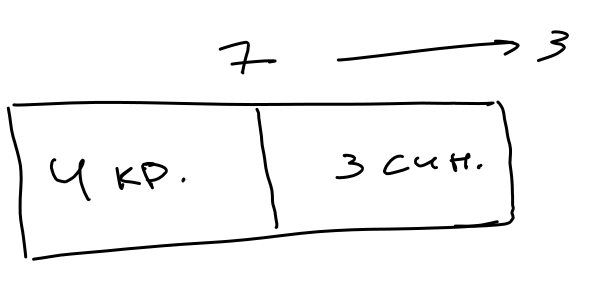
\includegraphics[width=.9\linewidth]{1_2.png}
\end{center}

\[ n = C^3_7 = \frac{7!}{3!4!} = \frac{5\cdot 6 \cdot 7}{2 \cdot 3} = 35 \]
\[ m = C^2_7 \cdto C^1_3 = 6\cdot 3 = 18 \]
\[ P(A) = \frac{m}{n} = \frac{18}{35} \]

\subsection{Задача 3}
\label{sec:orgda34c75}
В ящике 5 черных шаров и 3 белых и 2 красных. Вынули половину их них. Какова вероятность что из них 2 белых и два черных

\begin{center}
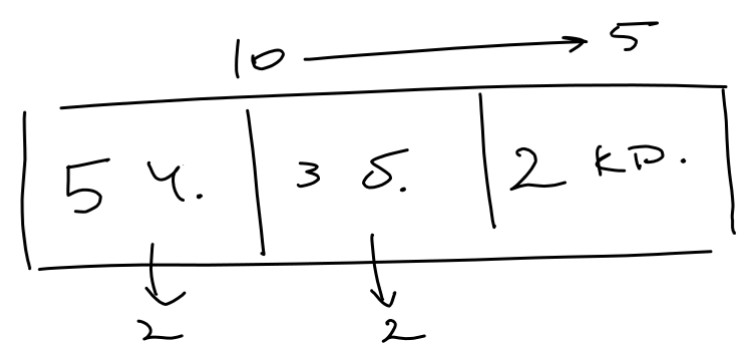
\includegraphics[width=.9\linewidth]{1_3.png}
\end{center}

\[ n = C^5_{10} = 252 \]
\[ m = C^2_5C^2_3 ?? \]


\subsection{Задача 4}
\label{sec:orgfc433ec}
В электричке 6 вагонов. Двое знакомых сели в электричку

\[ n = 6^2 \]
\[ m = 6 \]
\[ P(A) = \frac{6}{36} = \frac{1}{6} \]

\subsection{Задача 5}
\label{sec:org24f823b}
На первом этаже 6-ти этажного дома зашли 5 человек. Какова вероятность что они выйдут на разных этажах.

Учитывем порядок
\[ n = 5^3 = 125 \]
Размещения \(A^m_n = \frac{n!}{(m - n)!}\)
\[ m =  A^3_5 = 5\cdot 4\cdot 3 = 60 \]
\[ P(A) = \frac{60}{125} = \frac{12}{25} \]

\subsection{Задача 6}
\label{sec:org6d5b105}
На полке расставляются 8 книг. Найти вероятность что 3 конкретные книги будут стоять рядом.

\begin{center}

\includegraphics[width=.9\linewidth]{1_6.png}
\end{center}

\[ n = 8! \]
Подобрали позицию для первой(6), 
\[ m = 6 \cdot 3!\cdot 5! \]

\subsection{Задача 7}
\label{sec:orged2e592}
За круглым садятся 5 человек. Вероятность что 2 конкретных человека окажутся рядом.

\[ n = 5! \]
\[ m = 5\cdot 2! \cdot 3! \]

\subsection{Задача 8}
\label{sec:orgdbdbba5}
На доске поставили белую и черную ладью. Вероятность что они не будут бить друг друга
\[ n = 64 \cdot 63 \]
\[ m = 64\cdot(64 - 15) \]

\subsection{Задача 9}
\label{sec:org58be12b}
8 комманд. Найти вероятность что две сильнейших команды окажутся в разных подгруппах

\begin{center}
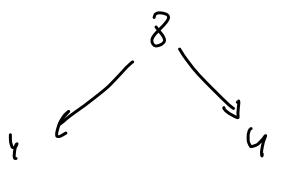
\includegraphics[scale=0.5]{1_8.png}
\end{center}

\[ n = C^4_8\cdot 1 = 70 \]
\[ m = C^1_2\cdot C^3_6 \cdot 1 \]

\subsection{Задача 10}
\label{sec:org257165a}
Бросается два кубика. Найти вероятность что в сумме не менее 9 очков

\begin{center}
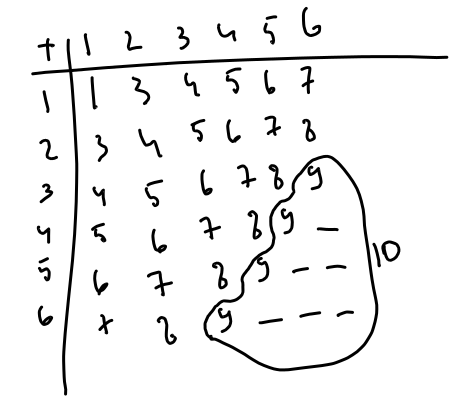
\includegraphics[scale=0.5]{1_11.png}
\end{center}

\[ n = 6^2 \]
\[ m = 10 \]

\subsection{Задача 11}
\label{sec:org7d6ad1c}
?? Карточек. Вероятность что осмысленное слово

\section{ДЗ}
\label{sec:orgaf1aab6}
\subsection{Задача 1}
\label{sec:org9b4e7e6}
В коробке 4 красных, 3 синих, 2 желтых карандаша. Вынули 6 карандашей. Найти веротяность что среди них поровну каждого цвета
\subsection{Задача 2}
\label{sec:org5f0b86a}
Карточки. Всего козырей 8. Известно что у двух человек 4 козыря. Найти вероятность что они распределились в соотношении:
\begin{enumerate}
\item 2 - 2
\item 3 - 1 (1 - 3)
\item 4 - 0 (0 - 4)
\end{enumerate}
\end{document}
